%%%%%%%%%%%%%%%%%%%%%%%%%%%%%%%%%%%%%%%%%
% University/School Laboratory Report
% LaTeX Template
% Version 4.0 (March 21, 2022)
%
% This template originates from:
% https://www.LaTeXTemplates.com
%
% Authors:
% Vel (vel@latextemplates.com)
% Linux and Unix Users Group at Virginia Tech Wiki
%
% License:
% CC BY-NC-SA 4.0 (https://creativecommons.org/licenses/by-nc-sa/4.0/)
%
%%%%%%%%%%%%%%%%%%%%%%%%%%%%%%%%%%%%%%%%%

%----------------------------------------------------------------------------------------
%	PACKAGES AND DOCUMENT CONFIGURATIONS

\documentclass[
	letterpaper, % Paper size, specify a4paper (A4) or letterpaper (US letter)
	10pt, % Default font size, specify 10pt, 11pt or 12pt
]{CSUniSchoolLabReport}

\addbibresource{sample.bib} % Bibliography file (located in the same folder as the template)

%----------------------------------------------------------------------------------------
\usepackage{geometry}
\usepackage{amsmath}
\usepackage{bm}
\geometry{a4paper, top = 2.2cm, bottom = 2.2cm, left=3.2cm, right=3.2cm}


%----------------------------------------------------------------------------------------
%	REPORT INFORMATION
%----------------------------------------------------------------------------------------

\title{Formulation of Lane Lines 2D to 3D Inverse Perspective Mapping (IPM)} % Report title

\author{Smart Automobile, Inc.} % Author name(s), add additional authors like: '\& James \textsc{Smith}'

\date{\today} % Date of the report

%----------------------------------------------------------------------------------------

\begin{document}

\maketitle % Insert the title, author and date using the information specified above


% If you need to include an abstract, uncomment the lines below
%\begin{abstract}
%	Abstract text
%\end{abstract}

%----------------------------------------------------------------------------------------
%	OBJECTIVE
%----------------------------------------------------------------------------------------

\section{Problem}
Figure 1 illustrates three coordinate systems: ego frame (i.e., the world coordinate system $\mathcal{F}_w$), camera frame $\mathcal{F}_w$ and image pixel coordinate system $\mathcal{F}_i$. When lane lines are detected in 2D images via deep learning models, the most challenging task is to inverse project the points of lane lines into world coordinate system $\mathcal{F}_w$.


\begin{figure}[H] % [H] forces the figure to be placed exactly where it appears in the text
	\centering % Horizontally center the figure
	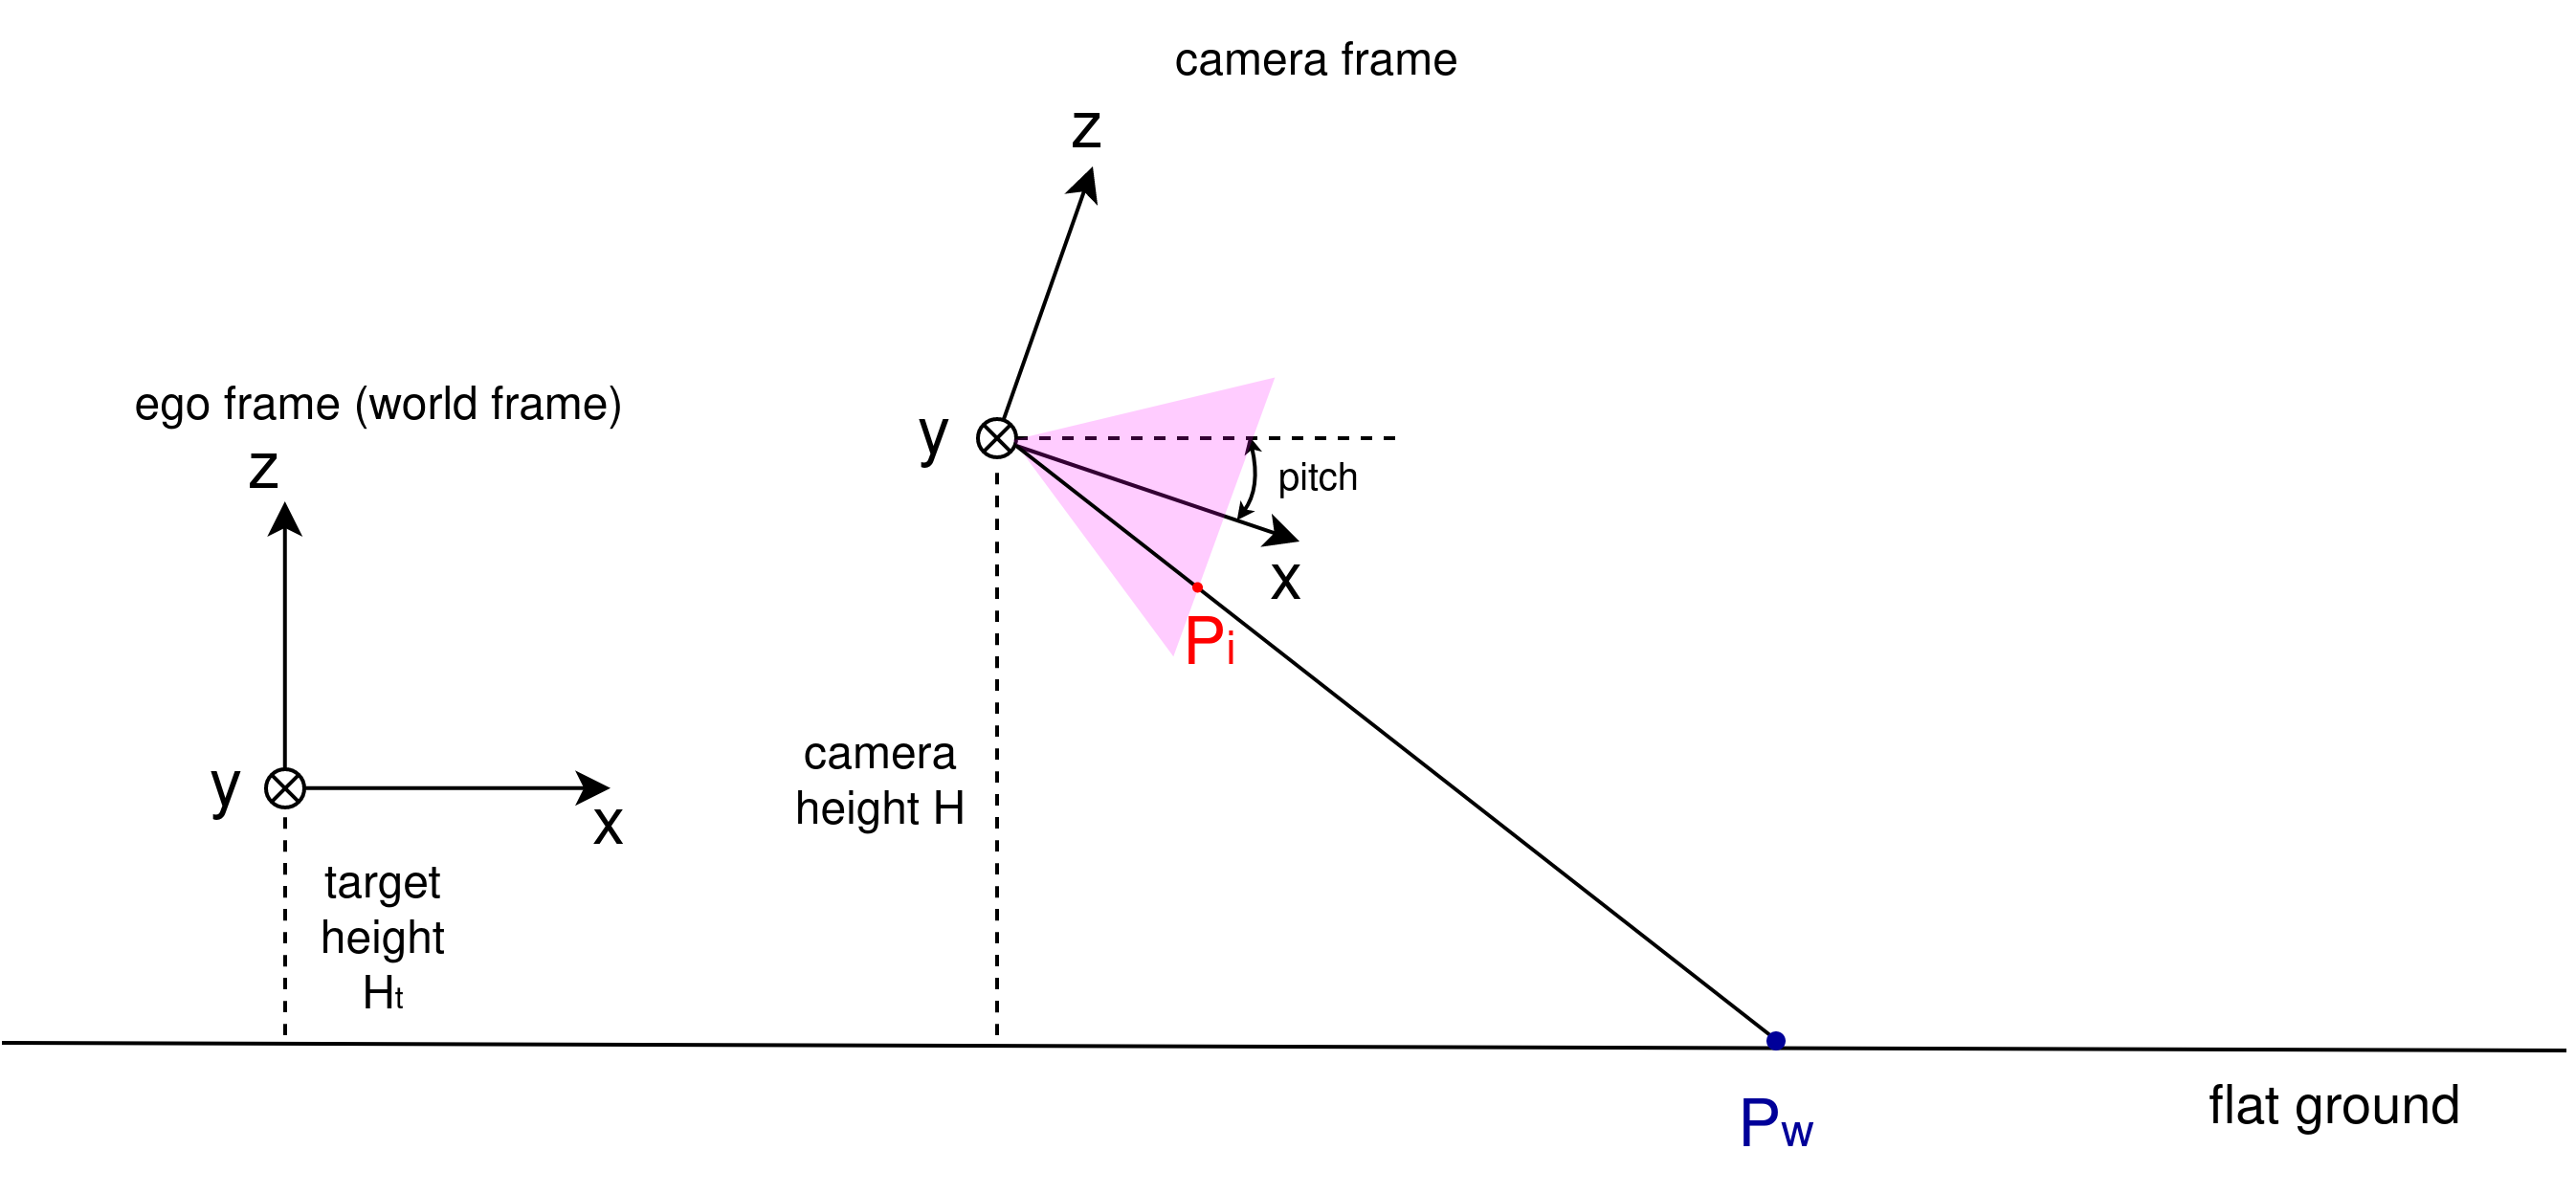
\includegraphics[width=0.95\textwidth]{IPM.png} % Include the figure
	\caption{Illustration of ego frame, camera frame and camera pose.}
\end{figure}

\section{Notation}
Consider a pixel point of lane lines in image plane $P_i = (u, v, 1)^T$, its corresponding 3D point in camera frame is noted as $P_c = (x_c, y_c, z_c)^T$ and its representation in ego frame is $P_w = (x_w, z_w, z_w)^T$. \\

The rotation matrix from world frame to camera frame is represented as $\bm{R}_{3\times 3}$.\\
The position of camera frame's origin point in world frame is represented as $\bm{T}_{3\times 1}$.\\
The camera intrinsic matrix is represented as $\bm{I}_{3\times 3}$.\\


\section{Formualation}
Follow the camera extrinisc and intrinsic model, the relationship between $P_w$ and $P_c$, $P_c$ and $P_i$ are formulated as:
\begin{equation}
P_c = \bm{R}_{3\times 3} P_w - \bm{T}_{3\times 1}
\end{equation}

\begin{equation}
P_i = \frac{1}{z_c}\bm{I}_{3\times 3} P_c
\end{equation}

respectively. Combine Equation 1 and 2, we can obtain:
\begin{equation}
z_c \begin{bmatrix}
u \\
v \\
1
\end{bmatrix} = \bm{I}_{3\times 3}\bm{R}_{3\times 3} \begin{bmatrix}
x_w \\
y_w \\
z_w
\end{bmatrix} - \bm{I}_{3\times 3}\bm{T}_{3\times 1}
\end{equation} \\

Therefore, 
\begin{equation}
\bm{R}^{-1}_{3\times 3}\bm{I}^{-1}_{3\times 3}\left(z_c \begin{bmatrix}
u \\
v \\
1
\end{bmatrix} + \bm{I}_{3\times 3}\bm{T}_{3\times 1} \right) = \begin{bmatrix}
x_w \\
y_w \\
z_w
\end{bmatrix}
\end{equation}

In the equation above, it is worth mentioning that the extrinsic matrix $\bm{R}_{3\times 3}$, 
$\bm{T}_{3\times 1}$ and the camera intrisic matrix $\bm{I}_{3\times 3}$ are calibirated in advance and already known. However, the depth $z_c$ is unknown and it is crital for calculating $P_w$. \\

We introduce three assumptions:\\
1. the ground plane is extremely flat; \\
2. the ego frame's $XY-plane$ is parallel with ground; \\
3. the origin point of ego frame is with height $H_t$ with respect to ground. \\

Then, we could config $z_w$ in Equation 4 to $-H_t$, we represent $\bm{R}^{-1}_{3\times 3}\bm{I}^{-1}_{3\times 3}$ and $\bm{I}_{3\times 3}\bm{T}_{3\times 1}$ as below:
\begin{equation}
\bm{R}^{-1}_{3\times 3}\bm{I}^{-1}_{3\times 3} = \begin{bmatrix}
a_{11} & a_{12} & a_{13} \\
a_{21} & a_{22} & a_{23} \\
a_{31} & a_{32} & a_{33} 
\end{bmatrix}, \bm{I}_{3\times 3}\bm{T}_{3\times 1} = \begin{bmatrix}
b1 \\
b2 \\
b3
\end{bmatrix}
\end{equation}

Combine Equation 5 and Equation 4 with condition $z_w = -H_t$, we can obtain:
\begin{equation}
z_c(a_{31}u + a_{32}v + a_{33}) = -H_t - b_3
\end{equation} 

i.e, the depth $z_c$ is:
\begin{equation}
z_c = \frac{-H_t - b_3}{a_{31}u + a_{32}v + a_{33}}
\end{equation} \\

After $z_c$ is calculated, then the corresponding point $P_w$ could be easily obtained with Equation 4.




\printbibliography % Output the bibliography

%----------------------------------------------------------------------------------------

\end{document}